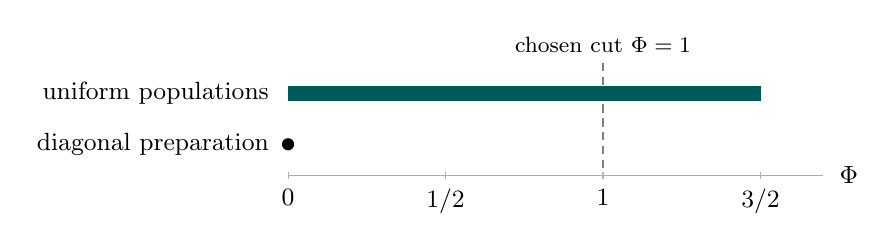
\begin{tikzpicture}[x=4cm,y=0.72cm,font=\small]
\draw[gray!65] (0,0)--(1.7,0);
\foreach \x/\v in {0/0,0.5/{1/2},1/1,1.5/{3/2}} {
 \draw[gray!60] (\x,-.06)--(\x,.06);
 \node[below] at (\x,-.07) {$\v$};}
\draw[densely dashed,gray] (1,.13)--(1,2.0);
\node[above,font=\footnotesize] at (1,2.0) {chosen cut $\Phi=1$};
\node[left] at (-.03,1.45) {uniform populations};
\node[left] at (-.03,.55) {diagonal preparation};
\fill[teal!70!black] (0,1.32) rectangle (1.5,1.58);
\fill[black] (0,.55) circle[radius=2.2pt];
\node[right] at (1.72,0) {$\Phi$};
\end{tikzpicture}
